\documentclass[UTF8,a4paper]{ctexart}
\usepackage{algorithm}
\usepackage{algorithmic}
\usepackage{verbatim}
\usepackage{comment}
\usepackage{amsmath}
\usepackage{graphicx}  %插入图片
\usepackage{amsfonts} % \mathbb{R}
\usepackage[numbers]{natbib} %参考文献
\usepackage{multicol} %分栏
\usepackage{color} %字体颜色

\usepackage{geometry} % 页边距
\geometry{a4paper,left=2cm,right=2cm,top=2cm,bottom=2cm} 

\renewcommand{\algorithmicrequire}{ \textbf{Input:}} %Use Input in the format of Algorithm
\renewcommand{\algorithmicensure}{ \textbf{Output:}} %UseOutput in the format of Algorithm
\renewcommand{\refname}{Reference} %把section标题改掉

\title{LDP机制下快速的频繁模式挖掘方法}
\author{王家礼}
%\date{\today}

\begin{document}
\maketitle

%\begin{multicols}{2}

\section{简介}
目前,本地化差分隐私主要研究方向有频率估计、均值估计、heavy hitter、频繁模式挖掘和键值数据收集等。其中,对频繁模式挖掘的工作相对较少,文献\cite{qin2016heavy}首次提出LDPMiner方法解决set-Valued场景下本地化数据聚合,并将频繁模式挖掘任务作为开放性问题提出,并没有实际解决该问题。由于本地化差分隐私具有强隐私保护性,任意第三方不会持有用户的敏感数据,所以,如何在噪声数据上进行频繁模式挖掘,并且同时保证LDP的隐私性以及估计结果的有效性,成为了当前一大难点问题。文献\cite{wang2018locally}首次提出了基于频率推测的候选集构造SVSM方法,其解决了频繁模式挖掘top-k问题。该方法的缺点在于,随着$k$值得不断增大,频率推测构造候选集的额外开销明细增大(详见\ref{computation}节),极大得限制了方法的应用。 

为了解决SVSM方法额外开销的问题,本文通过引入FPgrowth\cite{han2000mining}模式挖掘算法,一方面实现了基于LDP的频繁模式挖掘方法,另一方面在挖掘结果有效的前提下,大大降低了所需的额外开销。

\textbf{本文贡献}:
\begin{enumerate}
  \item[1、]LDP机制下频繁模式树的层次建立;
  \item[2、]对模式树及挖掘结果的优化;
  \item[3、]大大降低SVSM\cite{wang2018locally}方法的额外计算开销。
\end{enumerate}

\section{背景知识介绍}
  \subsection{频繁模式挖掘}

  频繁模式是指频繁地出现在数据集中的模式,如:项集、子序列或子结构,本文主要针对频繁项集的挖掘(FIM问题)。自文献\cite{agrawal1994fast}首次研究在数据库中发掘项集,FIM已被广泛的研究。FIM任务的定义如下。给定一个用户交易数据库,FIM的目的是发掘数据库中频繁出现的项目和一起出现项目集合(项集)。

  \textbf{频繁项集挖掘(FIM)}:令$DB= \left\{ t_{1},t_{2},\ldots,t_{n}\right\}$表示$n$位用户的交易数据集,其中用户$u_{i}$的交易记录$t_{i} \subset I=\left\{x_{1}, x_{2}, \ldots, x_{d}\right\}$,$I$为总项目集合,$x_{j}$表示项目(或商品),$1 \leq i \leq n$,$1 \leq j \leq d$。FIM任务的结果在于挖掘出$DB$中所有频繁出现的项集。如图\ref{fig:1}所示,为$n=5,I=\{a,b,c,f,g,h,l,n,o,p\}$时的交易数据集。

  \begin{figure}[htbp]
  \begin{minipage}{0.5\linewidth}
    \centering
    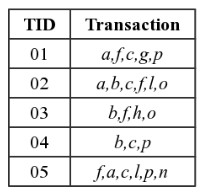
\includegraphics[width=0.4\textwidth]{DB}
    \caption{交易数据集}
    \label{fig:1}
  \end{minipage}
  \hfill %分栏
  \begin{minipage}{0.5\linewidth}
    \centering
    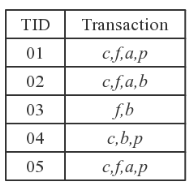
\includegraphics[width=0.4\textwidth]{2}
    \caption{预处理数据集}
    \label{figure:2}
  \end{minipage}
  \end{figure}

  %在建立模式树时,先扫描一次原始数据集(图\ref{fig:1})获得各项目的频数(即出现次数),如$a$出现3次、$f$出现4次。对各项目进行排序得到有序的项目序列为$c\prec f\prec a\prec b \prec p$,其他项目由于小于给定最低频数3,为非频繁项目,故舍弃。然后依据该序列,原始数据进行预处理:每个用户只保留频繁项目,且将保留项目以序列顺序进行排序,得到图\ref{figure:2}。最后根据图\ref{figure:2}数据集信息,建立频繁模式树如图\ref{figure:tree}。

  %\begin{figure}[h]
    %\centering
    %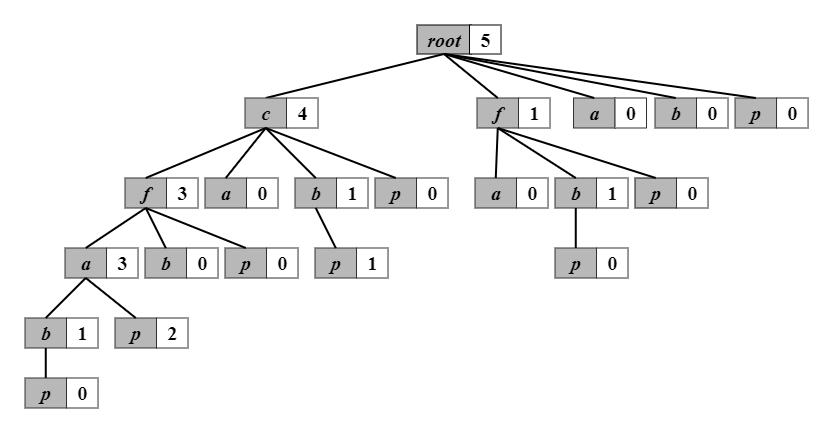
\includegraphics[width=0.9\textwidth]{tree}
    %\caption{模式树}
    %\label{figure:tree}
  %\end{figure}

  \textbf{定义、频繁项集($frequent\  itemset$)}:若$X\subset I$,则$X$表示一个项集。当其支持度(在数据集中出现次数)$support(X)$不低于给定阈值时,则$X$是一个频繁项集。

  \textbf{定义、$\alpha-itemset$}:项集$X$的项目个数记为$\alpha = \left | X \right |$,则$X$是一个$\alpha - itemset$。

  \subsubsection{FPgrowth模式挖掘方法\cite{han2000mining}}
  \label{fpgrowth}
  本节是对非隐私保护情况下,FPgrowth模式挖掘方法的简介。FPgrowth主要分为两个步骤:建立模式树存储用户信息和挖掘模式树获得频繁模式。

  \textbf{一、建立频繁模式树FP(本文主要工作是,在LDP场景下,构建有效的FP树)}

  \textbf{1、建立项头表} ——(第一次扫描数据集,得到项头表,也即频繁$1-itemset$)

  扫描交易数据集一遍,记录每个项出现的次数,根据给定的最小支持度计数(或最小支持度)筛选得到频繁$1-itemset$及它们的支持度计数,按计数值从大到小依次排序得到项头表。

  如:图\ref{fig:1}交易数据集(每行为一个交易),在给定最小支持度计数为3得到项头表如图\ref{fig:item_table}

  %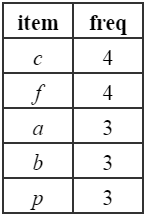
\includegraphics[width=0.2\textwidth]{item_table}

  \begin{figure}[htbp]
    \centering
    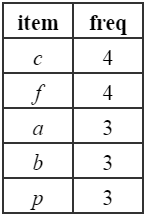
\includegraphics[width=0.15\textwidth]{item_table}
    \caption{项头表}
    \label{fig:item_table}
  \end{figure}

  \textbf{2、预处理数据集} ——(根据所得项头表,预处理数据集,将非频繁的项删除,只保留频繁的项,并且进行排序)
  
  因为原始的交易数据集中的交易可能包含频繁$1-itemset$中没有的项(即除项头表以外的项),所以对于每个事务要把非频繁$1-itemset$中的项过滤掉,同时为了方便FP树的建立,需要把每个交易中的项(过滤后)按照其支持度大小排序,得到新交易数据集。预处理后新的交易数据集如图\ref{figure:2}。

  \textbf{处理规则:}                                                            将原始的交易数据集中的每一个交易(每一行)删除项头表中没有的项,并且剩下项按照项头表中每一项的支持度计数从大到小排序(所有交易共用一个项目排序,$c,f,a,b,p$)。

  \textbf{3、FP树的建立} —— (第二次扫描数据集,根据每个处理后交易记录,构建模式树)

  1)、FP树的根节点默认为$root$,其相应的计数为总用户数$n$;

  2)、将新交易数据集中的每个交易变成FP树中的一条路径,并统计每个项出现的次数;

  3)、对于后插入的交易先从树的根节点开始找与其相同的部分,从第一个不重合的项开始建立一个新的分支。

  \textbf{例:新的交易数据集如图\ref{figure:2}}

  扫描第一个交易为{\color{red}$c,f,a,p$}:

  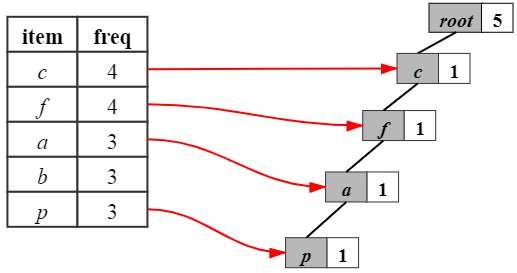
\includegraphics[width=0.4\textwidth]{1_trans}

  扫描第二个交易为{\color{red}$c,f,a,b$}:
  
  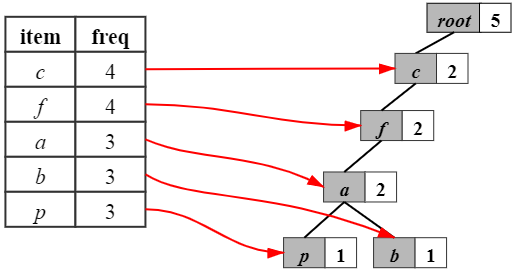
\includegraphics[width=0.4\textwidth]{2_trans}

  扫描第三个交易为{\color{red}$f,b$}:
  
  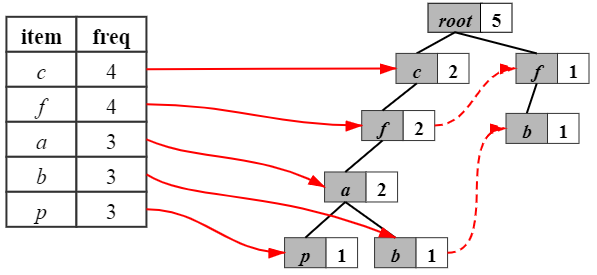
\includegraphics[width=0.47\textwidth]{3_trans}

  扫描第四个交易为{\color{red}$c,b,p$}:
  
  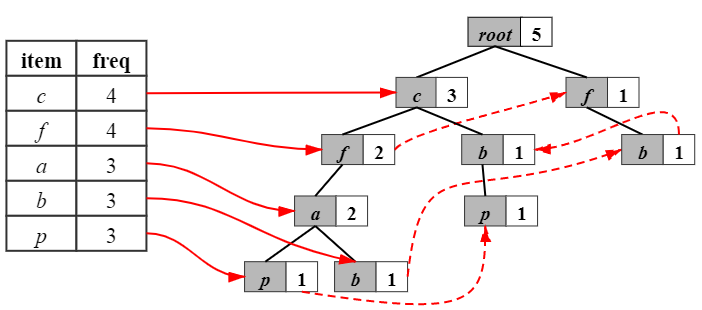
\includegraphics[width=0.55\textwidth]{4_trans}

  扫描第五个交易为{\color{red}$c,f,a,p$}:
  
  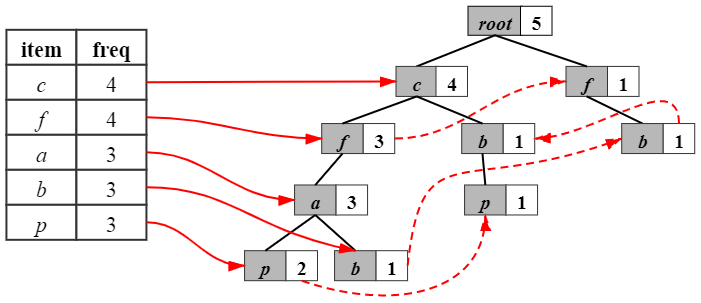
\includegraphics[width=0.55\textwidth]{5_trans}

  其中用项头表记录树中对应的项的节点位置,用以进行后续的挖掘步骤。

  \textbf{二、FP树的挖掘(本文直接使用该挖掘过程,未修改)}

  通过建立的FP树,从项头表的最后一项从下到上开始挖掘频繁项集。

  挖掘步骤:

  从项头表的最后一项从下到上开始,如当前项为$i$
  
  ①得到以$i$结尾的所有路径的前缀路径,前缀路径是指每个路径删掉该项后的路径。通常前缀路径的最后一项是一个数字,用来记录该路径出现的次数,该数字以项$i$的计数为准。

  如:项$a$的前缀路径为$(c,f,3)$,由以项F结尾的路径$(c,f,a)$删掉$a$得到,并且项$a$的计数为3,所以$(c,f,a)$路径出现的次数为3。

  ②根据项$i$的所有前缀路径得到条件模式基,条件模式基是将项$i$的所有前缀路径根据计数合并,过滤掉小于最小支持度的项。

  如:项$p$的前缀路径为$(c,f,a,2)$,$(c,b,1)$,根据$p$的前缀路径最后的计数很容得到前缀路径中每一项出现的次数$(c:2,f:2,a:2)$,$(c:1,b:1)$,然后将所有的前缀路径合并得到$(c:3,f:2,a:2,b:1)$,因为项目$f,a,b$的计数小于最小支持度计数3,所以将其过滤得到最终的条件模式基$(c:3)$

  ③根据项$i$的条件模式基画出项i的条件FP树。

  如{\color{red}项$p$的条件FP树为}:

  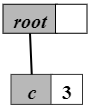
\includegraphics[width=0.1\textwidth]{p_baseTree}

  {\color{red}项$a$的条件FP树为}:

  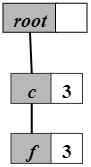
\includegraphics[width=0.1\textwidth]{a_baseTree}

  ④根据项$i$的条件FP树得到项 $i$ 的频繁项集。从左到右遍历项 $i$ 的条件FP树的每一条路径,用路径中的每单个节点和项 $i $组合得到项$ i $的频繁$2-itemset$,用路径中每2个节点与项 $i $组合得到频繁$3-itemset$,以此类推用路径中的每k个节点与项$ i$ 组合得到项$ i $的频繁$(k+1)-itemset$。

 如项$p$的频繁项集为:

 频繁$2-itemset$:$(c,p,3)$

 项$a$的频繁项集为:

 频繁$2-itemset$:$(c,a,3),(f,a,3)$

 频繁$3-itemset$:$(c,f,a,3)$


 ⑤继续挖掘剩余项的频繁项集,得到最小支持度为3的所有频繁项集结果为:
  $$(c,p,3),(c,a,3),(f,a,3),(c,b,3),(c,f,3),(c,f,a,3)$$

  \textbf{总结:}FPgrowth方法需要扫描两次原始数据集,分别用于建立项头表(频繁$1-itemset$)和建立模式树。

  \subsection{本地化差分隐私(LDP)}
  \textbf{LDP定义}

  \subsection{频数估计协议}
  LDP频数估计的目的是获得任意指定项目$x \in I = \left\{ x_{1},x_{2},\ldots,x_{d} \right\}$在$n$位用户中真实出现次数$\theta(x)$的无偏估计$\tilde{\theta}(x)$。

  \subsubsection{FO协议}
  \label{section:FO}
  最基本场景——每位用户的记录中只有一个项目$x$,最终估计所有项目的频数值$\tilde{\theta}(x)$

    \textbf{一、GRR(Generalized Randomized Response)}

    \textbf{用户端——扰动加噪}:

    $$
    {\forall}_{y \in I} Pr \big[ f_{GRR-\epsilon}(x) \big] =
    \begin{cases}
    p = \frac{e^{\epsilon}}{e^{\epsilon}+d-1},  & \text{if $y = x$ } \\
    q = \frac{1}{e^{\epsilon}+d-1},  & \text{if $y \neq x$} 
    \end{cases}
    \eqno{(2)}
    $$

    \textbf{第三方——统计聚合}:

    $$\tilde{\theta}_{GRR-\epsilon}(x) = \frac{C(x)-n\cdot q}{p-q} \eqno{(3)}$$

    \textbf{估计误差——方差}:

    $$Var \big[ \tilde{\theta}_{GRR-\epsilon}(x) \big] = n \cdot \frac{d-2+e^{\epsilon}}{(e^{\epsilon}-1)^{2}} \eqno{(4)}$$

    \textbf{二、OLH(Optimized Local Hashing)}
    为了改进GRR方法的估计误差与$d$呈线性关系的缺点,OLH使用$hash$函数将$d$映射到$g = \left \lceil e^{\epsilon}+1 \right \rceil$范围内,在$g$中使用GRR方法。

    \textbf{用户端——扰动加噪}:

    $$f_{OLH-\epsilon}(x) := \Big \langle hash , f_{GRR-\epsilon}\big(hash(x)\big) \Big \rangle \eqno{(5)} $$

    \textbf{第三方——统计聚合}:
    
    $$\tilde{\theta}_{OLH-\epsilon}(x) = \frac{C(x)-n/g}{p-1/g} \eqno{(6)}$$

    其中$g = \left \lceil e^{\epsilon}+1 \right \rceil , p = \frac{e^{\epsilon}}{e^{\epsilon}+g-1}$。

    \textbf{估计误差——方差}:

    $$Var \big[ \tilde{\theta}_{OLH-\epsilon}(x) \big] = n \cdot \frac{4 e^{\epsilon}}{(e^{\epsilon}-1)^{2}} \eqno{(7)}$$

    关于GRR与OLH的更详细介绍见文献\cite{wang2017locally}。由于FO协议是在用户记录仅有一个项目的情况,但是本文考虑set-valued\cite{qin2016heavy,wang2018locally}场景,即用户记录有多个项目且个数未知,所以文献\cite{wang2018locally}使用了PSFO协议(\ref{section:PSFO}节)。

  \subsubsection{PSFO协议——用户的项目个数未知且随机}
  \label{section:PSFO}
  本文场景——每位用户持有记录中有多个项目,并且个数未知且无规律,如图\ref{fig:1}所示为$n=5$位用户及其交易记录

  \textbf{填充或截取:Padding and Sampling(PS)}:给定一个正整数$l$和一条记录$V \subset I$,记$\perp_{1},\perp_{2},\ldots,\perp_{l} \not\in I$为$l$个无效值。$PS_{l}(V)$步骤如下:
  
  1、若$\left | V \right | < l$,则向$V$中随机添加(均匀随机)$l - \left | V \right |$个不同的无效值;若$\left | V \right | > l$,则在$V$中随机选择$l$个项目保留,其余项目丢弃;

  2、在处理之后的记录$V$中随机选择一个项目,并且输出该项目。

  PSFO协议即是先进行PS操作,然后以FO协议进行后续LDP聚合。后续FO协议的值域应为$I^{\prime} = I \cup \{ \perp_{1},\perp_{2},\ldots,\perp_{l}\}$,且第三方需要将FO协议的聚合结果乘以因子$l$,从而保证其为无偏估计。

  PSFO协议的形式表述为:

 $$PSFO(l,FO,\epsilon) := \Big \langle f_{FO-\epsilon}\big(PS_{l}(\cdot)\big), \tilde{\theta}_{FO-\epsilon}(\cdot)\times l \Big\rangle \eqno{(8)}$$

  \subsubsection{LDP机制下的$top-k$频繁模式聚合}
  在满足LDP隐私保证的同时,聚合有效的频繁模式,并且发布出$top-k$的频繁模式及其支持度。

  \subsection{现有方案}
    文献\cite{wang2018locally}首次提出LDP机制下的$top-k$频繁项集挖掘方法,分别为SVIM和SVSM。其中SVIM方法用于获得$top-k$的频繁$1-itemset$结果$S^{\prime}$(即LDP的$top-k$频率估计),然后利用所得$S^{\prime}$信息,通过SVSM方法获得$top-k$的$\alpha-itemset(\alpha > 1)$结果。然而,SVSM在进行$k$值较大时的挖掘任务时,会产生非常大的额外计算开销。所以,本文针对频繁项集挖掘任务,同样利用SVIM获得$S^{\prime}$,然后通过引入FPgrowth方法进行$\alpha-itemset(\alpha > 1)$挖掘任务。

    \subsubsection{方案介绍}    
    1、SVIM用于发布$top-k$的$1-itemset$(SVIM方法实现了LDP机制的$top-k$频率估计任务);

    2、SVSM用于发布$top-k$的$\alpha-itemset(\alpha > 1)$。

    \textbf{SVSM步骤:SVIM获得$1-itemset$结果$S^{\prime}\Rightarrow$ 以$S^{\prime}$构建并选择$top-2k$的候选集$IS \Rightarrow$ 以$IS$进行SVIM方法获得$top-k$的$\alpha-itemset(\alpha > 1)$。}\\


    \textbf{SVSM候选集$IS$构建——SVSM的主要步骤}

    $$\varphi(X)=\prod_{x \in X} \mu(x) , \mu(x) = \frac{0.9\times \tilde{\theta}(x)}{\max \limits_{x \in S^{\prime}} \tilde{\theta}(x)}\eqno{(9)}$$

    $x$为$S^{\prime}$中的某个项目,$\tilde{\theta}(x)$为$S^{\prime}$中项目$x$的估计频率。

    例:假设$k=4时$通过SVIM方法获得的$1-itemset$结果为$S^{\prime} = \{ c:4 , f:4, a:3, b:3\}$,则构建候选集$IS$步骤如下:

    1)计算$t = \lfloor \log_{2}k \rfloor = 2$;

    2)$k=4$个项目共计有$2^{k}$种组合,先筛选项目个数大于1且不小于$t$的组合,并且利用公式(9)分别组合的推测频数;如:通过计算组合$(c,f)$的推测频率为$0.81$、组合$(c,a)$的推测频率为$0.6075$
%即为$(c,f) , (c,a), (c,b), (f,a), (f,b), (a,b)$,

    3)以推测频率进行排序,选择频率的$top-2k$个组合作为候选集$IS$。

    \subsubsection{方案缺点}
    SVSM以SVIM的$top-k$频繁$1-itemset$结果$S^{\prime}$作为输入,然后使用公式(9)计算出所有可能项集的推测频数,用于构建出候选集$IS$。在$IS$的构建过程中,$k$个项目生成共计有$2^{k}-k$个$\alpha-itemset(\alpha>1)$项目集合

    $$2^{k} = \dbinom{k}{1} + \dbinom{k}{2} + \ldots + \dbinom{k}{t} + \ldots + \dbinom{k}{k}\eqno{(10)}$$

    而SVSM方法通过将$t$限制为$t = \lfloor \log_{2}k \rfloor$,保证其推测频数的计算空间为$O \left ( \dbinom{k}{2} + ... + \dbinom{k}{t} \right)$。然而,随着$k$值的增大,计算开销也会明显增大(详见\ref{computation}节)。

\section{本文工作}
通过SVSM方法的介绍可知,该方法在$k$值较大时,开销会很大。本文利用频繁模式树对用户数据的压缩存储特性,结合FPgrowth的挖掘算法,实现了快速且高效的LDP模式挖掘方法。总体流程如算法\ref{alg:fullstep}所示。

\begin{algorithm}[htbp]
    \caption{LDP建树总步骤}
    \label{alg:fullstep}
        \begin{algorithmic}[1]
        \REQUIRE ~~\\
        $n$位用户的交易数据集 $\mathrm{DB}=\left\{t_{1}, t_{2}, \ldots, t_{n}\right\}$;\\
        $d$个项目组成的值域$I=\left\{x_{1}, x_{2}, \ldots, x_{d}\right\}$;\\
        正整数$k$;隐私预算$\epsilon$;
        \ENSURE $top-k$的频繁项集
        \STATE 将数据集$DB$按比例分为三个互斥的子组$D B_{1}$、$D B_{2}$和$D B_{3}$: \\
            $\left|D B_{1}\right|=n_{1}=0.5 n,\left|D B_{2}\right|=n_{2}=0.1 n,\left|D B_{3}\right|=n_{3}=0.4 n$
        \label{fullstep:group}
	   \STATE $D B_{1}$的用户执行$SVIM$方法得到$top-k$频繁$1-itemset$集合\\
	       $S^{\prime}=\left\{x^{1}: \tilde{\theta}^{1}, x^{2}: \tilde{\theta}^{2}, \ldots, x^{k}: \tilde{\theta}^{k}\right\}$
        \label{fullstep:SVIM}
        \FOR{each $t_{j} \in D B_{2} \cup D B_{3}$}
        \label{fullstep:for}
        \STATE //预处理数据集
        \STATE $t=t_{j} \cap S$;
        \STATE 以$S^{\prime}$中项目顺序对$t$进行排序;
        \STATE 将处理后的记录$t$作为用户$j$的隐私数据;
        \ENDFOR
        \label{fullstep:endfor}

        \STATE M = 算法\ref{alg:iter}估计最大迭代次数($D B_{2}$,$k$,$\epsilon$);
        \label{fullstep:MaxIter}
        \STATE tree = 算法\ref{alg:bulid tree}建树($D B_{3}$,$S^{\prime}$,$\epsilon$,M);
        \label{fullstep:tree}
        \STATE $top-k$ = FPgrowth(tree); //挖掘过程详见文献
        \label{fullstep:mine}
        \STATE 对$top-k$结果进行优化;//见\ref{section:weight}节
        \label{fullstep:post process}
        \RETURN $top-k$
        \end{algorithmic}
\end{algorithm}

\textbf{算法\ref{alg:fullstep}简介}

步骤\ref{fullstep:group}使用分组的方式将总用户分为三组,让不同的组内用户以全部隐私预算参与不同的聚合过程,\ref{section:Q3}节所述,这样会降低误差;

步骤\ref{fullstep:SVIM}利用SVIM方法在LDP场景下聚合$top-k$的$1-itemset$集合$S^{\prime}=\left\{x^{1}: \tilde{\theta}^{1}, x^{2}: \tilde{\theta}^{2}, \ldots, x^{k}: \tilde{\theta}^{2}\right\}$,然后公开S的信息;

步骤\ref{fullstep:for}至\ref{fullstep:endfor}的目的是将用户原始记录中非频繁的项目剪枝删除,因为频繁项集的Apriori属性,非频繁项目,不可能产生频繁项集,故删除是合理的;

步骤\ref{fullstep:MaxIter}进行最大迭代次数的估计,即树的最大深度估计,见\ref{section:Q4}节;

步骤\ref{fullstep:tree}是本文主要工作部分,即在LDP场景下建立频繁模式树,详见\ref{setction:buildtree}节;

步骤\ref{fullstep:mine}是对模式树的挖掘过程,由于过程于文献\cite{han2000mining}相同,故不详细介绍。

步骤\ref{fullstep:post process}是差分隐私的后处理步骤,不消耗隐私预算,也不会泄露用户隐私。\\
\\
\textbf{总结}:算法\ref{alg:fullstep}是整个机制的总体流程,步骤\ref{fullstep:SVIM}与步骤\ref{fullstep:MaxIter}过程与文献\cite{wang2018locally}所用方法相似,为已有方法;本文只是在步骤\ref{fullstep:MaxIter}时,修改了部分参数的值,具体如下:

1、长度估计时,SVIM设置参数$\gamma=0.9$,本文设置$\gamma=0.8$用于估计树的最大深度;

2、在临界值的设置中,SVIM设置$\mathrm{T}=F^{-1}\left(1-\frac{0.05}{2 k}\right) \sqrt{V a r}$,其中$F$为标准正态分布的CDF,将所得的估计结果不大于T的记为无效估计,令为0;本文设置$T=\frac{\sqrt{n}}{\epsilon}$,祥见\ref{section:Q4}节。


    \subsection{LDP机制下的频繁模式树层次建立}
    \label{setction:buildtree}
    根据算法\ref{alg:fullstep}可知,建立频繁模式树的前提,是在已知$1-itemset$结果$S^{\prime}$,以及预处理之后的数据集$DB^{\prime}$,即以图\ref{figure:2}所示数据记录建立模式树,LDP场景下的建树步骤具体如下:(记树中根节点为第$level = 0$层,向下依次递增)
    
1、初始化树的根节点$root$,为树的$level=0$层;

2、第$level=1$层树节点聚合;对预处理后的交易记录进行一次LDP频率估计,如下

如用户$u_{1}$预处理后的交易为{\color{red}$c,f,a,p$},则其当前阶段的隐私信息为其前$level=1$个项,即为$c$;

用户$u_{2}$预处理后的交易为{\color{red}$c,f,a,b$},则其隐私信息为$c$;

用户$u_{3}$预处理后的交易为{\color{red}$f,b$},则其隐私信息为$f$;用户$u_{4}$的隐私信息为$c$;用户$u_{5}$的隐私信息为$c$。

则经过第三方聚合后,得到结果为$\{(c,4),(f,1)\}$,然后建第$level=1$层树节点,如图\ref{figure:levelone}所示,其中由于FO协议的特性,需要已知聚合的值域,也就是当前层的所有可能节点(见\ref{section:Q1}),图中计数为0的节点为无效节点。

  \begin{figure}[h]
    \centering
    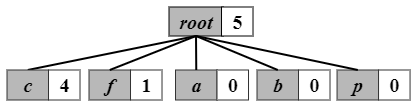
\includegraphics[width=0.5\textwidth]{level_1}
    \caption{第1层树节点}
    \label{figure:levelone}
  \end{figure}

3、第$level=2$层树节点聚合;

用户$u_{1}$预处理后的交易为{\color{red}$c,f,a,p$},则其当前阶段的隐私信息为其前$level=2$个项,即为$(c,f)$;

用户$u_{2}$的隐私信息为$(c,f)$,用户$u_{3}$的隐私信息为$(f,b)$,用户$u_{4}$的隐私信息为$(c,b)$,用户$u_{5}$的隐私信息为$(c,f)$

第三方聚合结果为$\left \{ (c,f,3) , (c,b,1) , (f,b,1) \right \}$,根据路径建立第$level=2$层树节点,如图\ref{figure:leveltwo}所示:

  \begin{figure}[h]
    \centering
    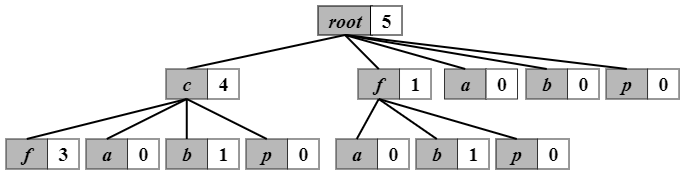
\includegraphics[width=0.8\textwidth]{level_2}
    \caption{第2层树节点}
    \label{figure:leveltwo}
  \end{figure}

4、依层次$level$递增顺序,直到达到树的最大层数,建立模式树如图\ref{figure:tree}所示。

  \begin{figure}[!]
    \centering
    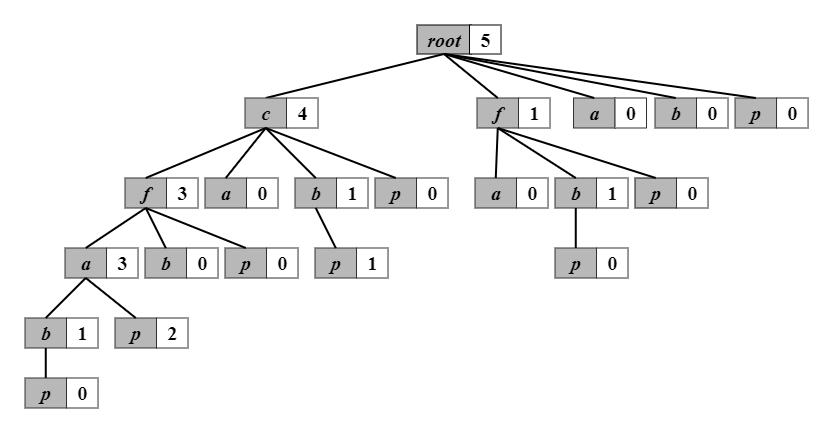
\includegraphics[width=0.9\textwidth]{tree}
    \caption{模式树}
    \label{figure:tree}
  \end{figure}

\textbf{总结}:算法\ref{alg:bulid tree}为层次建树具体过程。

\begin{algorithm}[htbp]
\caption{建树}
\label{alg:bulid tree}
\begin{algorithmic}[1]
\REQUIRE ~~\\
频繁$1-itemset$集合$S^{\prime}=\left\{x^{1}: \tilde{\theta}^{1}, x^{2}: \tilde{\theta}^{2}, \ldots, x^{k}: \tilde{\theta}^{2}\right\}$;\\
预处理后的数据集$D B^{\prime}_{3}$;\\
正整数$k$;隐私预算$\epsilon$;\\
最大迭代次数$M$;
\ENSURE 模式树

\STATE 初始化树根结点$root$为空;
\STATE 初始化候选值域$I^{\prime}_{1}$为$S^{\prime}$中项目,作为第一层次的LDP聚合值域;
\STATE 将$D B^{\prime}_{3}$均分为$M$个人数相同的子组~~\\
$G_{1},G_{2},...,G_{M};$
\STATE 初始化FO协议标准差为$standard\_error$ ;

\FOR{层次$j=1$ to $M$}
    \STATE FO协议聚合$estimation = Aggregate(I^{\prime}_{j},j,G_{j})$;\\
    //用户使用前$level$个项目参与,若无记录,则以无效值$\perp$参与。
    \STATE 删除$estimation$中估计值不大于$standard\_error$的结果;\\
    //无效值$\perp$不用于建树。
    \STATE 以$estimation$聚合结果更新第$j$层树$root$节点;
    \STATE 根据第$j$层节点,生成所有可能的孩子节点,作为下一层初始值域$I_{j+1}$;
    \STATE $I^{\prime}_{j+1} = \text{算法\ref{alg:prune}}(I_{j+1},S^{\prime},k,\xi)$
\ENDFOR

\RETURN $root$
\end{algorithmic}
\end{algorithm}

\textbf{存在问题}:上述建树过程仍然存在以下问题,对问题的具体解决过程见下文:
\begin{enumerate}
  \item[Q1、]LDP机制下如何进行每层节点的频数聚合;
  \item[Q2、]set-valued场景用户记录长度不固定且随机,聚合过程中,用户记录可能为空;
  \item[Q3、]隐私预算$\epsilon$的分配;
  \item[Q4、]树的最大层次。
\end{enumerate}


%\section{问题的解决}
%本节介绍了前文中所述问题的具体优化。
  \subsection{Q1——模式树的LDP机制下层次建立}
  \label{section:Q1}
  在使用FO频率估计协议进行当前第$j$层数据聚合时,首先需要解决的问题是如何确定输出值域$I_{j}$?

  %由LDP的FO协议特性可知,需要的已知条件有,输出值域$I$、隐私预算$\epsilon$。则用户可以根据本地数据,在输出值域$I$上扰动从而得到噪声数据。由于隐私预算$\epsilon$是已知的,所以问题的关键在于,输出值域$I$的确定。\textbf{即问题转化为,在第$j$层树节点计数聚合时,输出值域$I_{j}$该如何确定?}

  \textbf{基本方法}
  由模式树层次建立的特性,第$j$层节点的信息,不仅与FO协议的聚合结果相关,而且与第$j-1$层保留的节点有关(因为无效节点不会产生下一层的节点)。所以,一种生成$I_j$的直接方法是依据第$j-1$层保留节点的信息,生成所有可能的孩子节点作为$j$层初始节点,然后将其作为$I_j$使用FO协议聚合。

  以图\ref{figure:tree}为例,第$0$层初始为根节点$root$

  当$j = 1$时,其上一层为根节点,则$I_1$初始为所有$1-itemset$,即$I_1 = \left\{ (c), (f), (a), (b) , (p)\right\}$;

  当$j = 2$时,第$1$层保留的有效节点为$\left\{(c),(f) \right\}$,所有可能的孩子节点路径为$\left\{(c,f),(c,a),(c,b),(c,p),(f,a),(f,b),(f,p)\right\}$即为$I_2$;($1-itemset$的项目顺序为$c,f,a,b,p$,模式树中的节点的孩子,对应项目的顺序要小于其父节点对应项目)

  同理可得,$I_3 =\left\{(c,f,a),(c,f,b),(c,f,p),(c,b,p) \right\}$,$I_4 = \left\{ (c,f,a,b),(c,f,a,p)\right\}$ ,$I_5 = \left\{ (c,f,a,b,p)\right\}$ 
  
  \textbf{优化方法}

  上述方法的缺点在于,当$S^{\prime}$中的项目增多或者上一层保留节点个数较多时,进行下一层节点聚合所得值域的大小$\| I_j\| = d_j$会明显变大。而LDP的FO协议的估计精确度与$d_j$呈正相关,如GRR方法的估计方差与$d_j$为线性关系,而OLH方法的方差虽然与$d_j$无关,但是其使用了$hash$函数将$d_j$映射到$g = \left \lceil e^{\epsilon}+1 \right \rceil$范围,随着$d_j$的增大,在进行统计时,$hash$碰撞也会明显增多,导致精确度的降低。
  
  为了减小$d_j$,从而提高估计准确度,本文提出值域筛选的进一步方法,将$d_j$进一步限制在大小为$3k \ll d_j$,且整个过程不消耗隐私预算。\textbf{详见\ref{section:prune candidate}节。}

  \subsection{Q2——用户记录为空或项目个数少于当前树的层次}
  \label{section:Q2}
  若用户在当前阶段的记录项目个数小于层次$j$或所得值域$I_j$中不包含用户的记录,那么,则该用户以给定无效值$\perp$为原始数据进行扰动,然后提交扰动结果。此时的值域则为$I_j \cup \perp$

  \subsection{Q3——隐私预算分配}
  \label{section:Q3}
  文献\cite{wang2018privtrie}指出,若给定最大迭代次数$M$,可将用户分为$M$个互不相交的小组,每组以全部隐私预算$\epsilon$参与一次聚合过程,且不重复参与。(\textbf{对于$M$的确定,见\ref{section:Q4}节})

  其同时指出,上述分配方式,与均分隐私预算为$\epsilon/M$,用户参与所有过程($M$次)的方式相比,减小了误差为$O(\sqrt{M})$倍.

  \subsection{Q4——树最大层次}
  \label{section:Q4}
  若不考虑用户隐私,最大迭代次数即为用户预处理后的项目记录最大长度,如图\ref{figure:2}所示,记录最大长度为5,则树的最大层次为5(根结点为第0层)。

  但是由于记录的长度也属于敏感信息,在LDP机制下,由于长度是不固定且随机的。本文以FO协议,先对用户的记录长度进行一次聚合,从所得结果中确定最大层次。其过程与文献\cite{wang2018locally}中对$L$值的确定相似,本文对其中一些参数值做了修改,具体见算法\ref{alg:iter}。

\begin{algorithm}[h]
\caption{估计最大迭代次数}
\label{alg:iter}
\begin{algorithmic}[1]
\REQUIRE 预处理后的数据集$DB^{\prime}_{2}$;正整数$k$;隐私预算$\epsilon$;
\ENSURE 最大迭代次数

\STATE 初始化临界值$T=3.0 \cdot \frac{\sqrt{n}}{\epsilon}$; /*$n$为$DB^{\prime}_{2}$的用户总数*/
\label{T threshold}
\FOR{each $t_{i} \in DB^{\prime}_{2}$}
\STATE //用户端扰动
\STATE $x=\left|t_{i}\right|$;
\STATE 利用公式(5)得到扰动结果$y=f_{OLH-\epsilon}(x)$,然后将$y$提交给第三方;
\ENDFOR

\FOR{each $m \in\{1,2, \ldots, k\}$}
  \STATE //第三方聚合
  \STATE 利用公式(6)计算出长度为$m$的用户估计人数$\tilde{\theta}_{OLH-\epsilon}(m)$;
  \IF{$\tilde{\theta}_{OLH-\epsilon}(m) \leq T$}
    \STATE $\tilde{\theta}_{OLH-\epsilon}(m) = 0$;
  \ENDIF
\ENDFOR
t
\STATE 利用公式(8)在$\gamma=0.8$时的整数值$M$;
\label{gamma=0.8}
\RETURN 最大迭代次数$M$
\end{algorithmic}
\end{algorithm}


  类似文献\cite{wang2018privtrie}所设置最大误差方法,由伯恩斯坦不等式可得,OLH聚合算法,对任意项目$x$的估计频数$\tilde{C}(x)$与真实频数$C(x)$,以至少$1 - \beta$的概率,当$\lambda = O \left( \frac{\sqrt{n} \cdot \sqrt{\ln{(1/\beta)}}}{\epsilon} \right)$时,不等式$\left| \tilde{C}(x) - C(x) \right| < \lambda$成立。
  
  本文设置$T=3.0 \cdot \frac{\sqrt{n}}{\epsilon}$为最大误差临界值,用于筛选估计结果,见算法\ref{alg:iter}步骤\ref{T threshold}。

  算法\ref{alg:iter}步骤\ref{gamma=0.8}中,$\gamma=0.8$的取值时一个权衡,根据实际情况进去修改(文献\cite{wang2018locally}使用值为0.9)。若$\gamma$越大,迭代次数$M$越大,会保留更多的用户信息,其估计值的累计误差(均值平方误差)会降低,但是由于迭代次数的增多,结果的命中率会有所降低。

  %\subsection{误差边界}
  %\label{section:error bound}
  %对项目$X$其估计频数$\tilde{C}(x)$与真实频数$C(x)$,以至少$1-\beta$的概率,当$\lambda = O \left( \frac{\sqrt{n \cdot M} \cdot \sqrt{\ln{(1/\beta)}}}{\epsilon} \right)$时,不等式 $\left| \tilde{C}(x) - C(x) \right| < \lambda$成立。$n$为总用户数,$M$为最大迭代次数(树最大层次)。

  %\textbf{注:这是对项目的频数误差分析,如$x = a$时,$\tilde{C}(x)$表示项目$a$的估计频数。 但是当$x$表示项集时,如$x = \{ a , c\}$,这个误差边界怎么计算——项目误差边界的倍数?}

\section{优化}
本章介绍了对模式树构建方法的进一步优化过程

\subsection{值域筛选}
\label{section:prune candidate}
  本文最终目的在于发布$top-k$的频繁$\alpha -itemset(\alpha > 1)$结果,如\ref{section:Q1}节所述,值域大小直接影响着估计结果的准确度,本节详细介绍了对值域的进一步筛选过程。
  
  在值域筛选过程中,利用文献\cite{wang2018locally}的SVSM方法思想,即根据$1-itemset$结果计算项集$X$的推测频率(公式(9)),然后排序选择$top-2k$个结果作为候选集进行LDP的聚合。

  类似于上述方法,本文在进行第$j$层聚合时,对其初始值域$I_{j}$进行了一次的频数推测,然后筛选出$top- \xi \cdot k$个作为最终值域$I^{\prime}_{j}$(实验中$\xi = 3$)。由于在该过程中,初始值域$I_{j}$中项集的长度必然为$j$,即属于$j-itemset$,所以公式(9)可直接省略为 $\varphi(X)=\prod_{x \in X} \tilde{\theta}(x)$。具体过程见算法\ref{alg:prune}。
  
\begin{algorithm}[h]
\caption{值域筛选}
\label{alg:prune}
\begin{algorithmic}[1]
\REQUIRE ~~\\
候选值域$I_{j}$;\\
1-itemset结果$S^{\prime}$;\\
正整数$k$;\\
参数$\xi$;
\ENSURE 筛选后值域$I^{\prime}_{j}$

\IF{$I_{j}$的长度不大于$4k$}
    \STATE $I^{\prime}_{j} = I_{j}$;
\ELSE
    \STATE 初始化$I^{\prime}_{j} = \emptyset$;
    \FOR{each 项集$X \in I_{j}$}
        \STATE $\varphi(X)=\prod_{x \in X} \tilde{\theta}(x)$;    //$\tilde{\theta}(x)$为1-itemset集合$S$中估计频数值。
        \STATE $I^{\prime}_{j} = I^{\prime}_{j} \cup X$,并记录$\varphi(X)$
    \ENDFOR
    \STATE 以$\varphi(X)$为标准,对$I^{\prime}_{j}$中项集排序;
    \STATE 选择$top-\xi \cdot k$赋值给$I^{\prime}_{j}$
\ENDIF

\RETURN $I^{\prime}_{j}$
\end{algorithmic}
\end{algorithm}

\subsection{临界值设置}
\label{section:tree threshold}
根据\ref{section:prune candidate}节所述方法确定值域后,以FO协议聚合出该阶段用户的信息,即为树当前层节点所需保留的信息。然而由于估计误差的存在,聚合结果中存在许多无效的估计(如:估计频数为负数等),本文通过设置临界值$error$对聚合结果进一步筛选,将所有估计频数不大于$error$的结果删除。$error$值的设置一方面要尽可能多的删除无效节点,另一方面也要将有效节点尽可能多的保留。本文设置的误差临界值为$error = \sqrt{Var}$,即LDP聚合协议的估计标准差。

\textbf{(类似误差值的设置有三种方法:)}

1、$error_{1} = \sqrt{Var}$,即标准差;

2、文献\cite{wang2017locally,warner1965randomized,wang2018locally},$error_{2} = \mathrm{T}=F^{-1}\left(1-\frac{0.05}{2 k}\right) \sqrt{V a r}$,$F^{-1}$为标准正态分布的CDF的倒数。

3、文献\cite{wang2018privtrie},$error_{3} = 3.0 \cdot \frac{\sqrt{n}}{\epsilon}$,其根据伯恩斯坦不等式求得最大误差边界(\ref{section:Q4}节)

\textbf{(三者的关系为$error_{1} < error_{2} < error_{3}$)}

\subsection{约束推理——一致性矫正,该部分仍然达不到预期效果,导致具体实验结果的均值平方误差与对比方案相比偏高}
\label{section:consistency}
设$v$表示树中某节点,其相应的计数值为$v.count$,则对于节点$v$应有以下约束:\\
\begin{enumerate}
  \item[1)、]无偏估计:$\mathbb{E} \left [ \tilde{C}(v.count) \right ] = \mathbb{E} \left [ C(v.count) \right ]$;即对节点的计数值的估计保证无偏(FO协议)
  \item[2)、]父节点计数值不小于孩子节点计数之和,记$v.children$表示$v$的所有孩子节点集合,假设有$r$个:\\
  $$\mathbb{E} \left [ \tilde{C}(v.count) \right ] \ge \sum_{y \in v.children} \mathbb{E} \left [ \tilde{C}(y.count) \right ] \eqno{(11)}$$
\end{enumerate}

  文献\cite{hay2010boosting,wang2018privtrie,lee2014top}等均研究了不同场景下的约束推理方式,其中文献\cite{wang2018privtrie}对两次的聚合结果进行矫正,不适用于本文场景;而文献\cite{hay2010boosting,lee2014top}均是DP机制下的约束推理。


  \textbf{具体矫正步骤}:

  %设$Y = (y_{1},y_{2},\ldots ,y_{r})$表示节点$v$的所有孩子节点(设$r$个)相应计数值,矫正的目的在于计算新的向量$Y^{\prime}$使其与$Y$的L2范式最小(文献\cite{hay2010boosting,lee2014top}),形式化表示为:\\
  %$$\underset{Y^{\prime}}{\text{minimize}}  \left \| Y^{\prime} - Y \right \|^{2}_{2} \  ,\  subject to \left \| Y^{\prime} \right \| = v.count\eqno{(12)}$$

  %上式可根据拉格朗日求解法得到$Y^{\prime} = Y - \frac{1}{2}A \ , \ A = \frac{2(\sum{i=1}^{k}y_{i} - A)}{r}$,其中$r$表示$v$的孩子节点个数,$A = v.count$。

  %即,在更新当前第$j$层树节点的之后,若对于$j-1$层存在违背约束的节点,则根据上述结果进行一致性矫正。(上述结果与文献\cite{hay2010boosting}结果是相同的,本文这里省略了文献中对父节点的矫正——本文只矫正孩子节点,且利用拉格朗日求解,计算过程比文献简单。)

\subsection{加权组合}
\label{section:weight}
  根据本文算法构建模式树,以最小支持度为0对树使用FP-growth算法\cite{han2000mining}所得到的所有频繁项集结果(不含$1-itemset$)为$IS^{\prime} = \left \{ X_{1}:\tilde{\theta}(X_{1}) , X_{2}:\tilde{\theta}(X_{2})  , \ldots ,  X_{s}:\tilde{\theta}(X_{s}) \right \}$,共$s$个为模式树中挖掘的项集及其频数。文献\cite{wang2018locally}指出,对某项集$X$可通过公式(9)计算出其推测频数$\varphi(X)$,然后得到其相对顺序。

  本文同样利用该推测频数信息,对估计结果,进行进一步的优化:

  1、对频数结果加权组合

  $$ \tilde{\theta}^{\prime}(X) = \omega \cdot \tilde{\theta}(X) + (1 - \omega)\cdot \varphi(X)\eqno{(13)}$$

  2、以加权结果的$top-k$项集作为最终输出的项目集合

  %\textbf{最终输出}:先计算出$\varphi(X_{i})\left( {\forall} X_{i} \in IS^{\prime} \right)$,然后输出以$\varphi(\cdot)$排序的$top-k$结果,而结果中的频数值为$\tilde{\theta}^{\prime}(X)$。


%\end{multicols}

\section{实验}
\label{exeperiment}

  记$X_{estimate} = \{X_{1} , X_{2} , \ldots , X_{k}\}$与$X_{correct}$分布表示$top-k$估计结果与真实结果,则$X_{cap} = X_{estimate} \cap X_{correct}$表示算法正确命中的项集。\\


  \textbf{评价指标\cite{wang2018locally}}:
  
  1、\textbf{NCR}(命中率):\\
  $$NCR = \frac{\sum_{X \in X_{estimate}} q(X)}{\sum_{X \in X_{correct}} q(X)}$$

  其中$q(X)$是评分,文献\cite{wang2018locally}将其根据$X_{correct}$的排序,依次设置为$k , k-1 , \ldots , 1$,其他均为0。

  2、\textbf{MSE}(误差——均值平方误差):\\
  $$ MSE = \frac{1}{\left \| X_{cap} \right \|}\sum_{X \in X_{cap}} \left (\theta (X) - \tilde{\theta} (X) \right)^{2}$$

  其中$\theta (X)$与$\tilde{\theta} (X)$分布是$X$的真实频数与估计频数。\\


  \textbf{数据集}:

  1、\textbf{Kosarak}:990002位用户的网页点击数据,总项目个数为41270,用户平均项目长度8.0,最大项目长度2498。

  2、\textbf{BMS-POS}:515597位用户的商品购买数据,总项目个数为1657,用户平均项目长度6.5,最大项目长度164。

\subsection{计算开销}
\label{computation}
  以下对比的开销只针对在值域筛选的搜索空间(搜索空间内排序并筛选得到值域的额外计算开销),其中对比方案的搜索空间大小只与$k$有关,根据公式(9)计算得到,而本文方案的搜索空间是在实验过程中总搜索空间(本文方案搜索空间与$k,\epsilon$以及数据集都有关,其中$\epsilon$和数据集会影响树中每层节点的保留数,保留节点越多,搜索空间越大)。以下结果是在$\epsilon=2.0$时的搜索空间对比。

\begin{table}[h]
		\centering
		\begin{tabular}{l|ccc}\hline
                k&\multicolumn{2}{r}{计算开销}\\\hline
                &对比方案&\multicolumn{2}{c}{本文方案$(\epsilon=2)$}\\
                & &POS数据集&Kosarak数据集\\
			50&2369885.0&6100.4&5537.5\\
                75&219904690.0&12807.15&10916.0\\
			100&1271427795.0&22979.6&17107.0\\
                125&4935173650.0&33532.8&24959.5 \\
			150&309019152705.0&46129.3&33036.5\\\hline
		\end{tabular}
		\caption{开销对比}
		\label{tab:computation}
\end{table}

\begin{figure}[h]
  \centering
  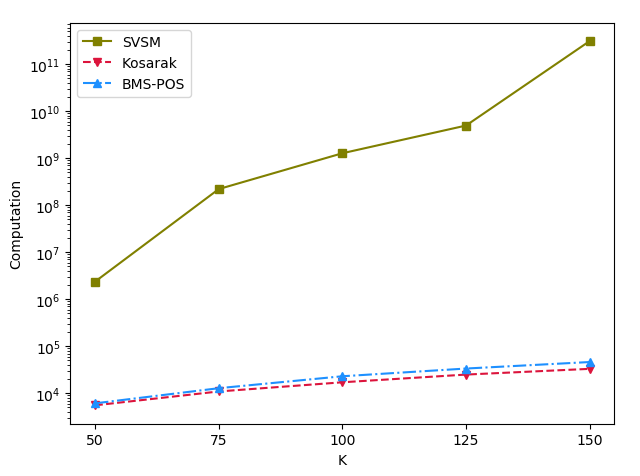
\includegraphics[width=0.6\textwidth]{computation}
  \caption{计算开销}
  \label{figure:computation}
\end{figure}

\newpage
\subsection{评分结果——该部分结果显示在高预算情况下,均值平方误差比对比方案高}
图中Origin线是未进行加权组合结果,即权值$\omega=1$;而SVSM线是本文的对比方案;Linear线是在$\omega=0.8$取值下的结果。

\textbf{Kosarak数据集}

  \begin{figure}[htbp]
    \centering
    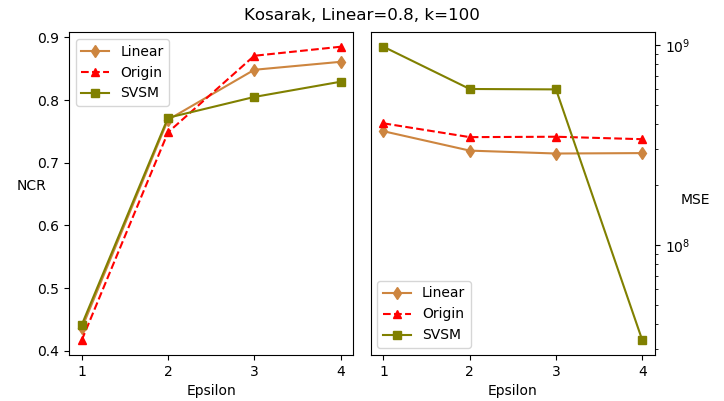
\includegraphics[width=0.845\textwidth]{kosarak_compare}
    \caption{Kosarak数据集,$Linear=0.8,k=100$时不同$\epsilon$对比}
    \label{fig:kosarak_compare}
  \end{figure}

  \begin{figure}[htbp]
    \centering
    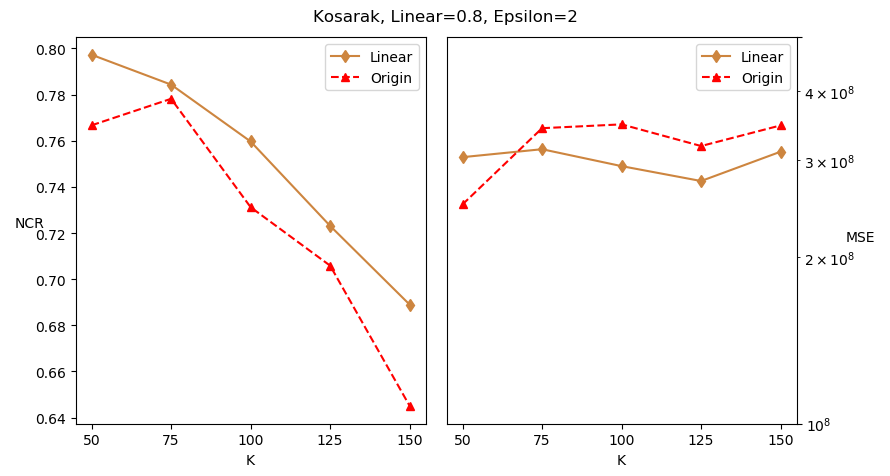
\includegraphics[width=0.845\textwidth]{kosarak_self}
    \caption{Kosarak数据集,$Linear=0.8,\epsilon=2$时不同$k$对比}
    \label{fig:kosarak_self}
  \end{figure}

\newpage
\textbf{BMS-POS数据集}

  \begin{figure}[htbp]
    \centering
    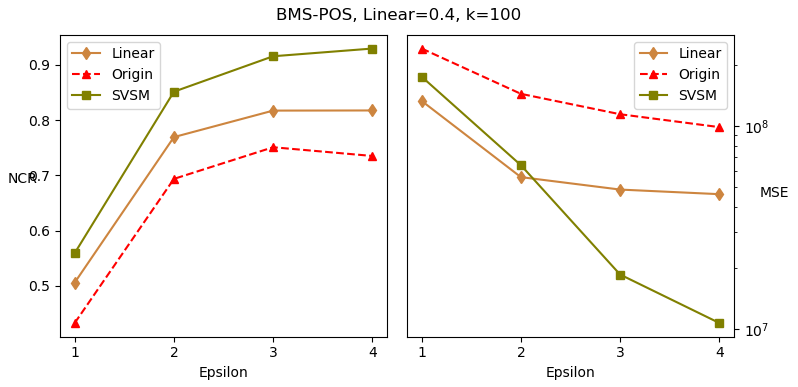
\includegraphics[width=0.8\textwidth]{pos_compare}
    \caption{BMS-POS数据集,$Linear=0.4,k=100$时方案对比}
    \label{fig:pos_compare}
  \end{figure}

  \begin{figure}[htbp]
    \centering
    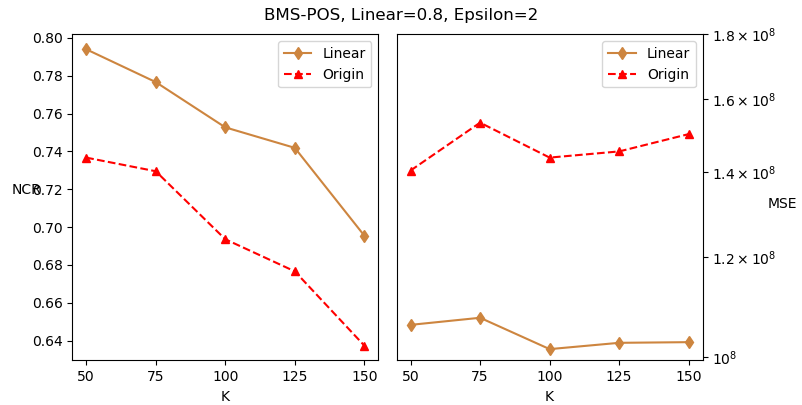
\includegraphics[width=0.8\textwidth]{pos_self}
    \caption{BMS-POS数据集,$Linear=0.8,\epsilon=2$时不同$k$对比}
    \label{fig:pos_self}
  \end{figure}

%\newpage
\subsection{加权组合}
图中Origin线是未进行加权组合结果,即权值$\omega=1$;而SVSM线是本文的对比方案;Linear线不同$\omega$取值下的结果。
\subsubsection{BMS-POS数据集不同$\epsilon$取值下的对比}

  \begin{figure}[htbp]
    \centering
    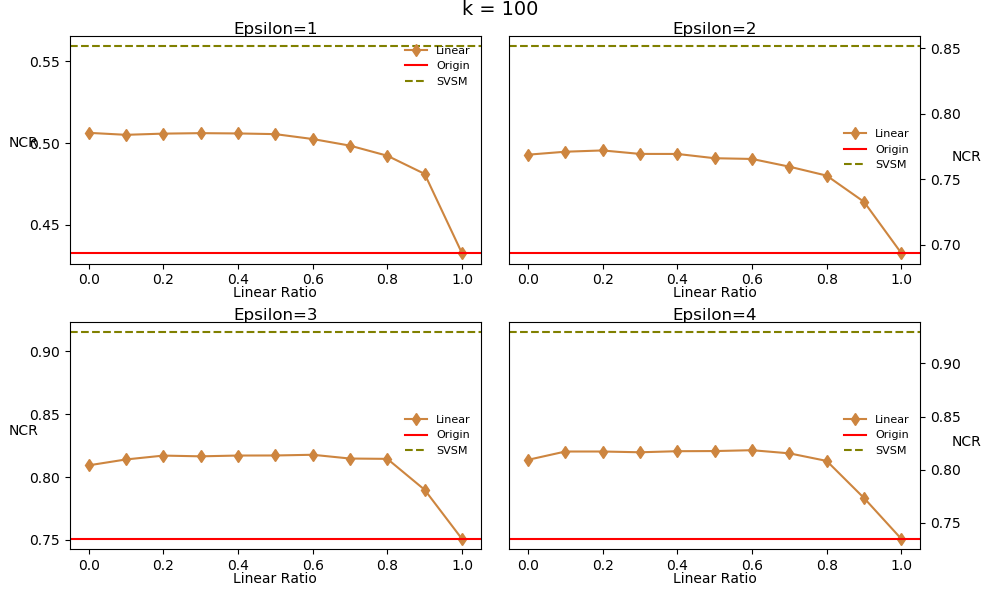
\includegraphics[width=0.85\textwidth]{pos_linear_ncr}
    \caption{BMS-POS命中率NCR对比}
    \label{fig:pos_linear_ncr}
  \end{figure}

  \begin{figure}[htbp]
    \centering
    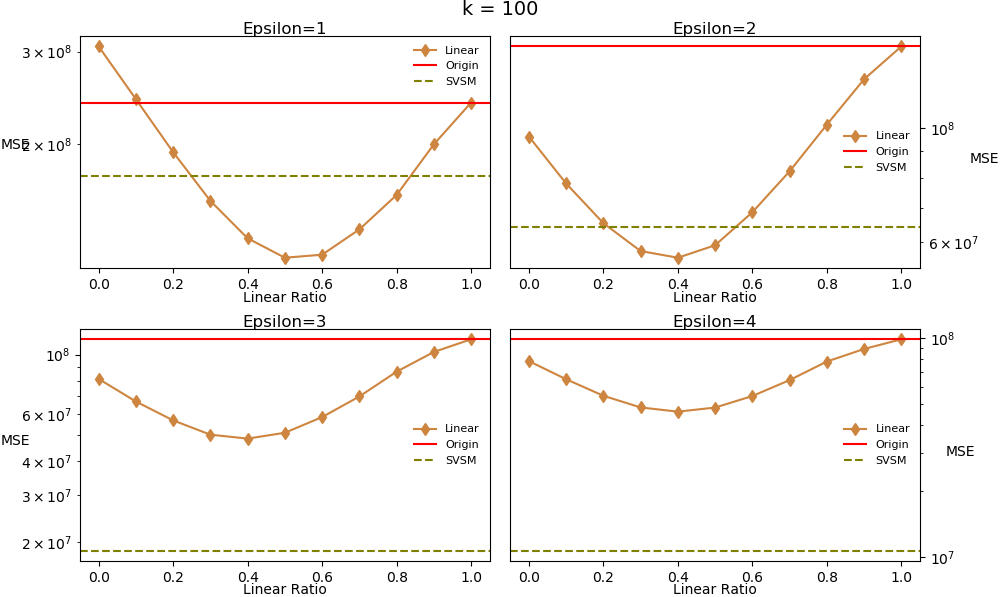
\includegraphics[width=0.85\textwidth]{pos_linear_mse}
    \caption{BMS-POS误差MSE对比}
    \label{fig:pos_linear_mse}
  \end{figure}

%图\ref{fig:pos_linear_ncr}可以看出,在不同$\epsilon$取值下,加权组合方法均可以提高最终的估计结果,然而依然比对比方案低,相差$10\%$;相同的,图\ref{fig:pos_linear_mse}中,在低$\epsilon$时,本文方法的误差低于对比方法,但是在$\epsilon$较高时,并没有其结果好。

\newpage
\subsubsection{Kosarak数据集不同$\epsilon$取值下的对比}
%图\ref{fig:kosarak_linear_ncr}中,命中率NCR与对比方案相差不大,约低$1\%$,而图\ref{fig:kosarak_linear_mse}误差在低$\epsilon$下会优于对比方案。

  \begin{figure}[htbp]
    \centering
    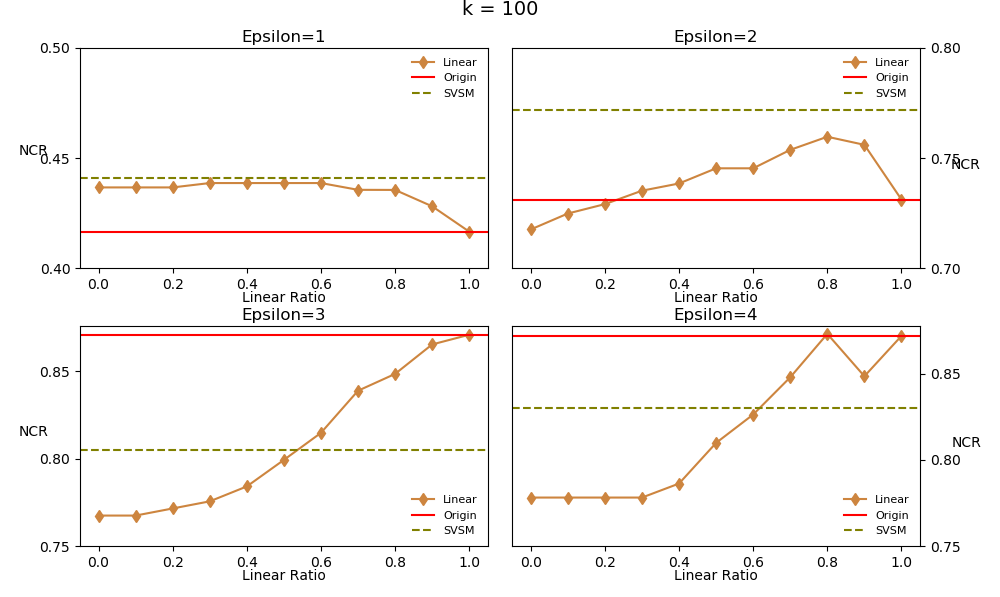
\includegraphics[width=0.85\textwidth]{kosarak_linear_ncr}
    \caption{Kosarak命中率NCR对比}
    \label{fig:kosarak_linear_ncr}
  \end{figure}

  \begin{figure}[htbp]
    \centering
    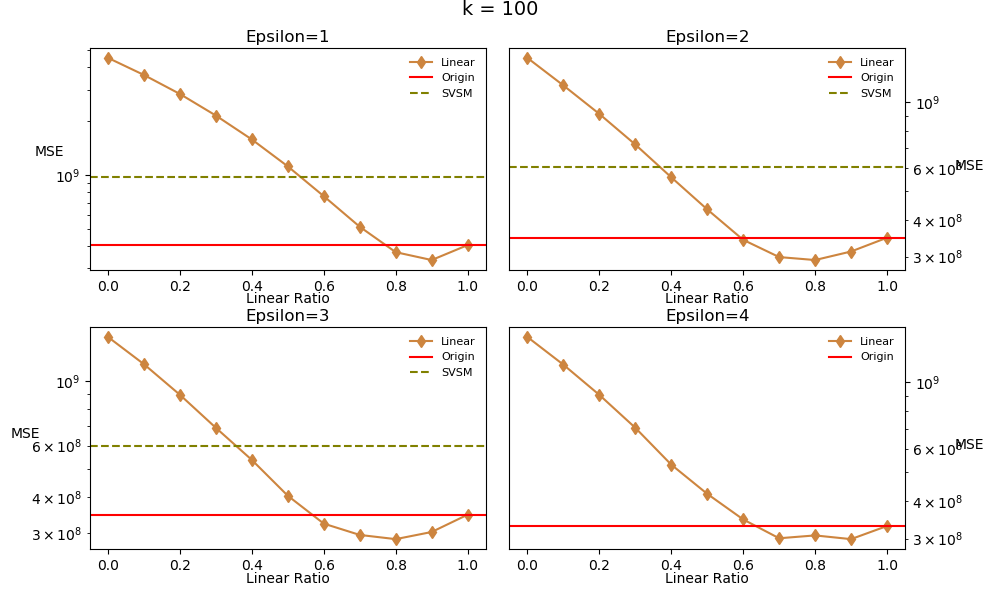
\includegraphics[width=0.85\textwidth]{kosarak_linear_mse}
    \caption{Kosarak误差MSE对比}
    \label{fig:kosarak_linear_mse}
  \end{figure}


%命中率NCR与误差MSE对比

  %\begin{figure}[h]
    %\centering
    %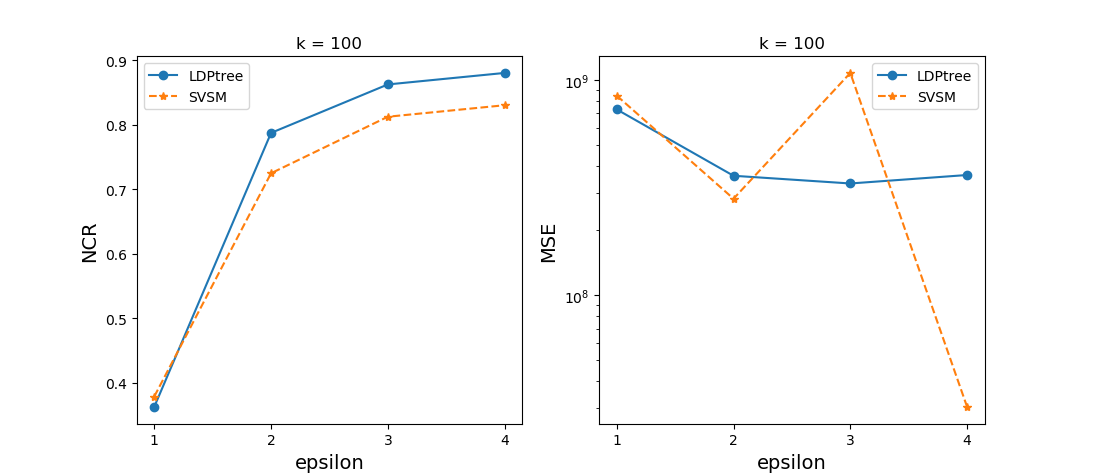
\includegraphics[width=0.9\textwidth]{kosarak}
    %\caption{kosarak数据集}
    %\label{figure:exe ko}
  %\end{figure}

  %\begin{figure}[h]
    %\centering
    %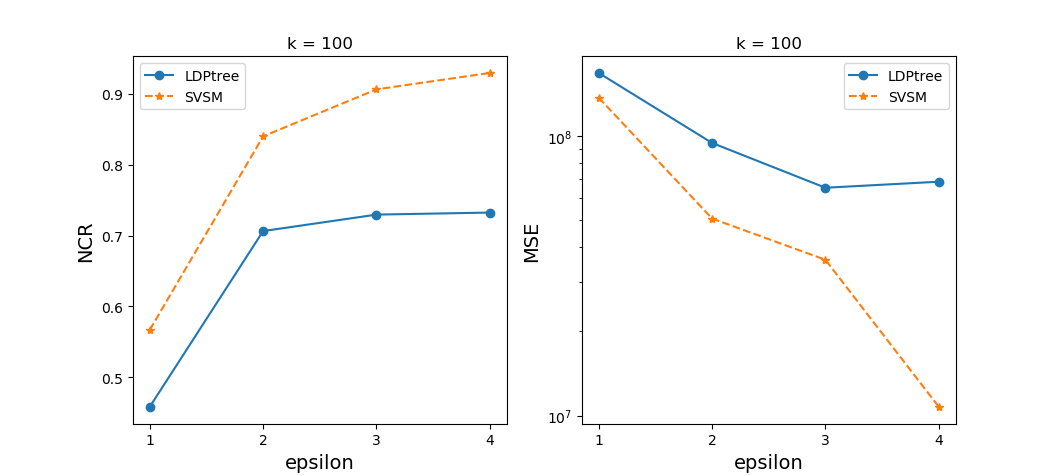
\includegraphics[width=0.9\textwidth]{pos}
    %\caption{pos数据集}
    %\label{figure:exe pos}
  %\end{figure}

%\newpage
%\subsection{加权组合}

  %\begin{figure}[h]
    %\centering
    %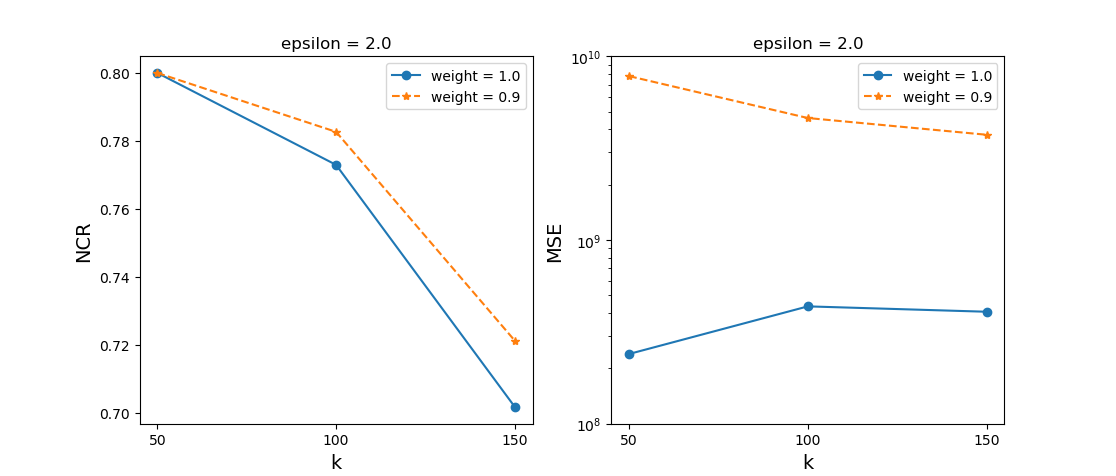
\includegraphics[width=0.9\textwidth]{ko_weight}
    %\caption{kosarak数据集加权}
    %\label{figure:exe ko weight}
  %\end{figure}

  %\begin{figure}[h]
    %\centering
    %\includegraphics[width=0.9\textwidth]{pos_weight}
    %\caption{pos数据集加权}
    %\label{figure:exe pos weight}
  %\end{figure}


\newpage
%设置文献的样式
\bibliographystyle{plainnat}      %unsrt表示PDF文末的参考文献列表是按照文中的引用顺序排序
%添加自己的bib文件
\newpage\bibliography{reference} 
\end{document}